\documentclass{article}
\usepackage{parskip}
\usepackage[utf8]{inputenc}
\usepackage{titlesec}
\usepackage[a4paper,top=2cm, bottom=2cm]{geometry}
\usepackage{tikz}
\usetikzlibrary{shapes}

\begin{document}
\section{Task}
    \subsection{How many disk blocks are used to store R and its B-tree?}
        $1$ diskblock $= 1$ node (with $100*0.7 = 70$ keys) \newline
        $1000000 / 70 = 14286$
        $\Rightarrow$ 14286 diskblocks
    \subsection{How many disk blocks are read on average to answer a point query matched by a single records given its search key?}
        sequential file $\Rightarrow$  $log_{70}(1000000) = 3.25$
    \subsection{How many disk blocks are read on average to answer a range query matched by 1,000 records?}
        $log_{70}(1000000) + 1000/70 = 17.53$
\section{Task}
    load data in file loaddata.sql with data from abc.csv \newline
    queries in file a8t2.sql

    \begin{tabular}{l l l}
        query & without index & with index \\
        \hline
        1 & 0.00049 & 0.000038 \\
        2 & 0.00025 & 0.000022 \\
        3 & 3.83487 & 0.001727 \\
        4 & 2.65559 & 0.001983 \\
    \end{tabular}

\section{Task}
\subsection{without rotation}
    insert 1

    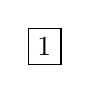
\begin{tikzpicture}
        \tikzstyle{bplus}=[rectangle split, rectangle split horizontal,rectangle split ignore empty parts,draw]
        \tikzstyle{every node}=[bplus]
        \node {1} 
    ;\end{tikzpicture}

    insert 2

    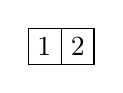
\begin{tikzpicture}
        \tikzstyle{bplus}=[rectangle split, rectangle split horizontal,rectangle split ignore empty parts,draw]
        \tikzstyle{every node}=[bplus]
        \tikzstyle{level 1}=[sibling distance=60mm]
        \node {1 \nodepart{two} 2}

    ;\end{tikzpicture}

    insert 3

    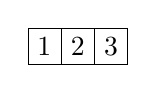
\begin{tikzpicture}
        \tikzstyle{bplus}=[rectangle split, rectangle split horizontal,rectangle split ignore empty parts,draw]
        \tikzstyle{every node}=[bplus]
        \node {1 \nodepart{two} 2 \nodepart{three} 3}
    ;\end{tikzpicture}

    insert 4

    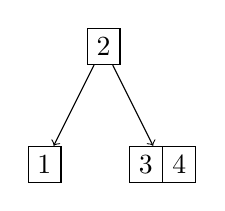
\begin{tikzpicture}
        \tikzstyle{bplus}=[rectangle split, rectangle split horizontal,rectangle split ignore empty parts,draw]
        \tikzstyle{every node}=[bplus]
        \node {2} [->]
        child {node {1}} 
        child {node {3 \nodepart{two} 4}} 
    ;\end{tikzpicture}

    insert 5

    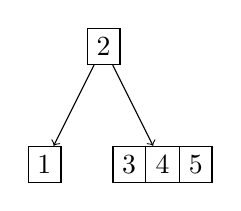
\begin{tikzpicture}
        \tikzstyle{bplus}=[rectangle split, rectangle split horizontal,rectangle split ignore empty parts,draw]
        \tikzstyle{every node}=[bplus]
        \node {2} [->]
        child {node {1}} 
        child {node {3 \nodepart{two} 4 \nodepart{three} 5}} 
    ;\end{tikzpicture}

    insert 6

    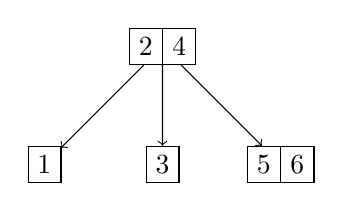
\begin{tikzpicture}
        \tikzstyle{bplus}=[rectangle split, rectangle split horizontal,rectangle split ignore empty parts,draw]
        \tikzstyle{every node}=[bplus]
        \node {2 \nodepart{two} 4} [->]
        child {node {1}} 
        child {node {3}}
        child {node {5 \nodepart{two} 6}}
    ;\end{tikzpicture}

    insert 7

    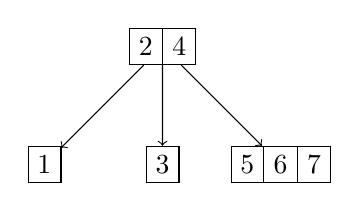
\begin{tikzpicture}
        \tikzstyle{bplus}=[rectangle split, rectangle split horizontal,rectangle split ignore empty parts,draw]
        \tikzstyle{every node}=[bplus]
        \node {2 \nodepart{two} 4} [->]
        child {node {1}} 
        child {node {3}}
        child {node {5 \nodepart{two} 6 \nodepart{three} 7}}
    ;\end{tikzpicture}

    insert 8

    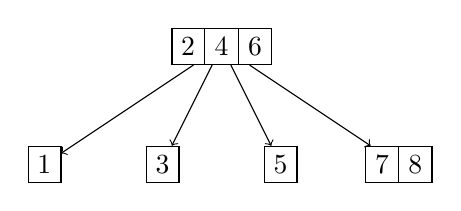
\begin{tikzpicture}
        \tikzstyle{bplus}=[rectangle split, rectangle split horizontal,rectangle split ignore empty parts,draw]
        \tikzstyle{every node}=[bplus]
        \node {2 \nodepart{two} 4 \nodepart{three} 6 } [->]
        child {node {1}} 
        child {node {3}}
        child {node {5}}
        child {node {7 \nodepart{two} 8}}
    ;\end{tikzpicture}

    insert 9

    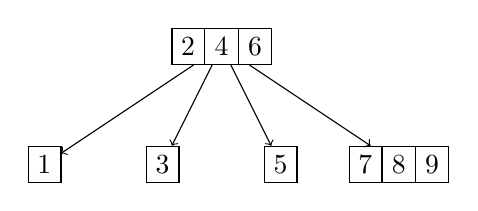
\begin{tikzpicture}
        \tikzstyle{bplus}=[rectangle split, rectangle split horizontal,rectangle split ignore empty parts,draw]
        \tikzstyle{every node}=[bplus]
        \node {2 \nodepart{two} 4 \nodepart{three} 6 } [->]
        child {node {1}} 
        child {node {3}}
        child {node {5}}
        child {node {7 \nodepart{two} 8 \nodepart{three} 9}}
    ;\end{tikzpicture}

    insert 10

    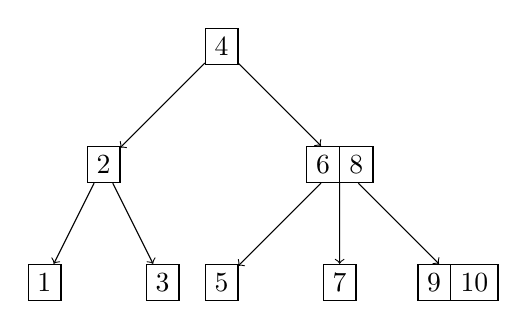
\begin{tikzpicture}
        \tikzstyle{bplus}=[rectangle split, rectangle split horizontal,rectangle split ignore empty parts,draw]
        \tikzstyle{every node}=[bplus]
        \tikzstyle{level 1}=[sibling distance=30mm]
        \tikzstyle{level 2}=[sibling distance=15mm]
        \node {4} [->]
        child {node {2} 
            child {node {1}}
            child {node {3}}
        }
        child {node {6 \nodepart{two} 8} 
            child {node {5}}
            child {node {7}}
            child {node {9 \nodepart{two} 10}}
        }
    ;\end{tikzpicture}

    \subsection{with rotation}
    insert 1

    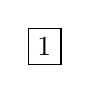
\begin{tikzpicture}
        \tikzstyle{bplus}=[rectangle split, rectangle split horizontal,rectangle split ignore empty parts,draw]
        \tikzstyle{every node}=[bplus]
        \node {1} 
    ;\end{tikzpicture}

    insert 2

    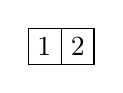
\begin{tikzpicture}
        \tikzstyle{bplus}=[rectangle split, rectangle split horizontal,rectangle split ignore empty parts,draw]
        \tikzstyle{every node}=[bplus]
        \tikzstyle{level 1}=[sibling distance=60mm]
        \node {1 \nodepart{two} 2}

    ;\end{tikzpicture}

    insert 3

    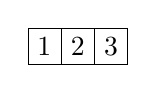
\begin{tikzpicture}
        \tikzstyle{bplus}=[rectangle split, rectangle split horizontal,rectangle split ignore empty parts,draw]
        \tikzstyle{every node}=[bplus]
        \node {1 \nodepart{two} 2 \nodepart{three} 3}
    ;\end{tikzpicture}

    insert 4

    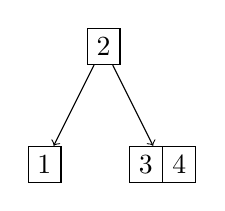
\begin{tikzpicture}
        \tikzstyle{bplus}=[rectangle split, rectangle split horizontal,rectangle split ignore empty parts,draw]
        \tikzstyle{every node}=[bplus]
        \node {2} [->]
        child {node {1}} 
        child {node {3 \nodepart{two} 4}} 
    ;\end{tikzpicture}

    insert 5

    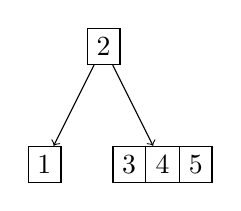
\begin{tikzpicture}
        \tikzstyle{bplus}=[rectangle split, rectangle split horizontal,rectangle split ignore empty parts,draw]
        \tikzstyle{every node}=[bplus]
        \node {2} [->]
        child {node {1}} 
        child {node {3 \nodepart{two} 4 \nodepart{three} 5}} 
    ;\end{tikzpicture}

    insert 6

    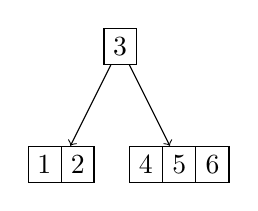
\begin{tikzpicture}
        \tikzstyle{bplus}=[rectangle split, rectangle split horizontal,rectangle split ignore empty parts,draw]
        \tikzstyle{every node}=[bplus]
        \node {3} [->]
        child {node {1 \nodepart{two} 2}} 
        child {node {4 \nodepart{two} 5 \nodepart{three} 6}}
    ;\end{tikzpicture}

    insert 7

    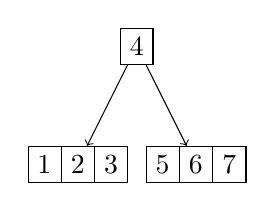
\begin{tikzpicture}
        \tikzstyle{bplus}=[rectangle split, rectangle split horizontal,rectangle split ignore empty parts,draw]
        \tikzstyle{every node}=[bplus]
        \node {4} [->]
        child {node {1 \nodepart{two} 2 \nodepart{three} 3}} 
        child {node {5 \nodepart{two} 6 \nodepart{three} 7}}
    ;\end{tikzpicture}

    insert 8

    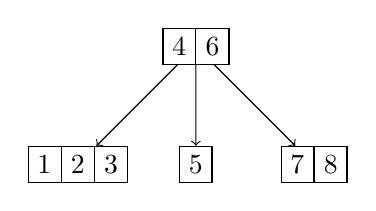
\begin{tikzpicture}
        \tikzstyle{bplus}=[rectangle split, rectangle split horizontal,rectangle split ignore empty parts,draw]
        \tikzstyle{every node}=[bplus]
        \node {4 \nodepart{two} 6} [->]
        child {node {1 \nodepart{two} 2 \nodepart{three} 3}} 
        child {node {5}}
        child {node {7 \nodepart{two} 8}}
    ;\end{tikzpicture}

    insert 9

    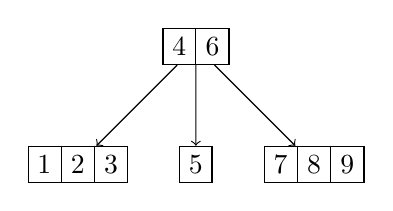
\begin{tikzpicture}
        \tikzstyle{bplus}=[rectangle split, rectangle split horizontal,rectangle split ignore empty parts,draw]
        \tikzstyle{every node}=[bplus]
        \node {4 \nodepart{two} 6} [->]
        child {node {1 \nodepart{two} 2 \nodepart{three} 3}} 
        child {node {5}}
        child {node {7 \nodepart{two} 8 \nodepart{three} 9}} 
    ;\end{tikzpicture}

    insert 10

    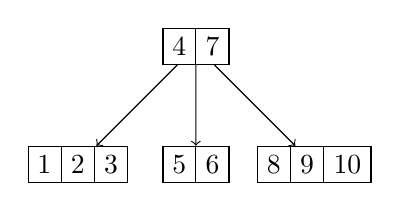
\begin{tikzpicture}
        \tikzstyle{bplus}=[rectangle split, rectangle split horizontal,rectangle split ignore empty parts,draw]
        \tikzstyle{every node}=[bplus]
        \node {4 \nodepart{two} 7} [->]
        child {node {1 \nodepart{two} 2 \nodepart{three} 3}} 
        child {node {5 \nodepart{two} 6}}
        child {node {8 \nodepart{two} 9 \nodepart{three} 10}} 
    ;\end{tikzpicture}
    
\end{document}